\begin{figure}
	\centering
	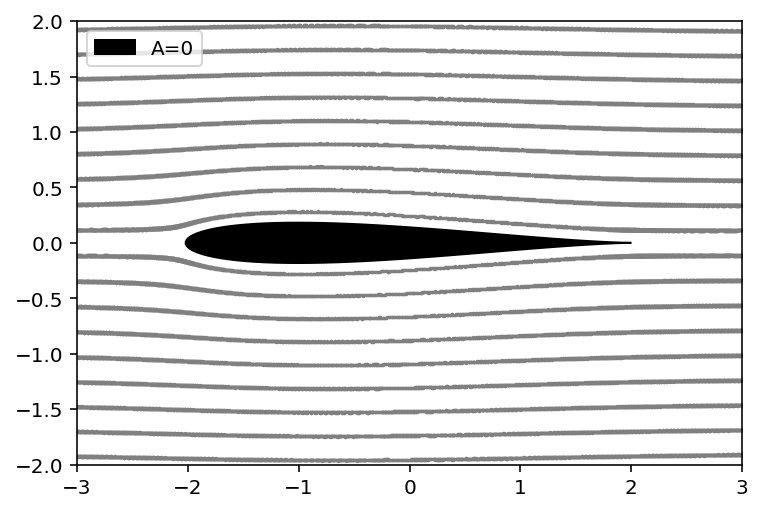
\includegraphics[width=0.6\textwidth]{papers/joukowski/images/05_stroemungslinien/fluegel_strom_A000_V04_g.png}
	\caption{
		Das flügelprofil ist in sich symmetrisch, was dazu führt dass die Strömungslinien auch symmetrisch verlaufen.
		Diese Anordnung produziert so keine Auftriebskraft.
		\label{joukowski:Stroemungslinien:fig_fluegel1}
	}
\end{figure}
